% =====================================================================
%  Chapitre 1 -- Donnees sequentielles : le probleme
%  Partie a : ouverture, types de sequences
% =====================================================================
\section{Chapitre 1 --- Données séquentielles}

\chapterslide{Chapitre 1}{Données séquentielles : le problème}%
{4 h --- texte, séries, signaux, trajectoires ; pourquoi l'ordre compte}%
{\textbf{Objectifs.} Reconnaître une donnée séquentielle ; transformer un texte en
nombres (tokens, embeddings) ; comprendre pourquoi MLP et CNN ne suffisent plus ;
poser le fil rouge du module : \textbf{prédire une trajectoire}.}

\begin{frame}{Plan du module}
\begin{columns}[t]
\begin{column}{0.48\textwidth}
\begin{kbox}[Les quatre temps]
\begin{enumerate}
  \item Les données séquentielles et leurs pièges.
  \item Le RNN : architecture, propagation, gradients.
  \item LSTM et GRU : dompter la mémoire.
  \item Entraînement, applications, projet.
\end{enumerate}
\end{kbox}
\end{column}
\begin{column}{0.48\textwidth}
\begin{ebox}[Ce que vous saurez faire]
\begin{itemize}
  \item Convertir un texte en tenseur exploitable.
  \item Écrire les équations d'une cellule récurrente.
  \item Expliquer le gradient qui s'évanouit par le calcul.
  \item Choisir entre RNN, GRU et LSTM en connaissance de cause.
\end{itemize}
\end{ebox}
\end{column}
\end{columns}
\vspace{1mm}
\begin{kbox}[Fil rouge du module]
Prédire la trajectoire d'une coccinelle à partir de ses positions passées ---
et classifier des critiques de films. Deux tâches, un même outillage.
\end{kbox}
\end{frame}

\begin{frame}{Une donnée séquentielle, c'est quoi ?}
\begin{columns}[t]
\begin{column}{0.55\textwidth}
\centering
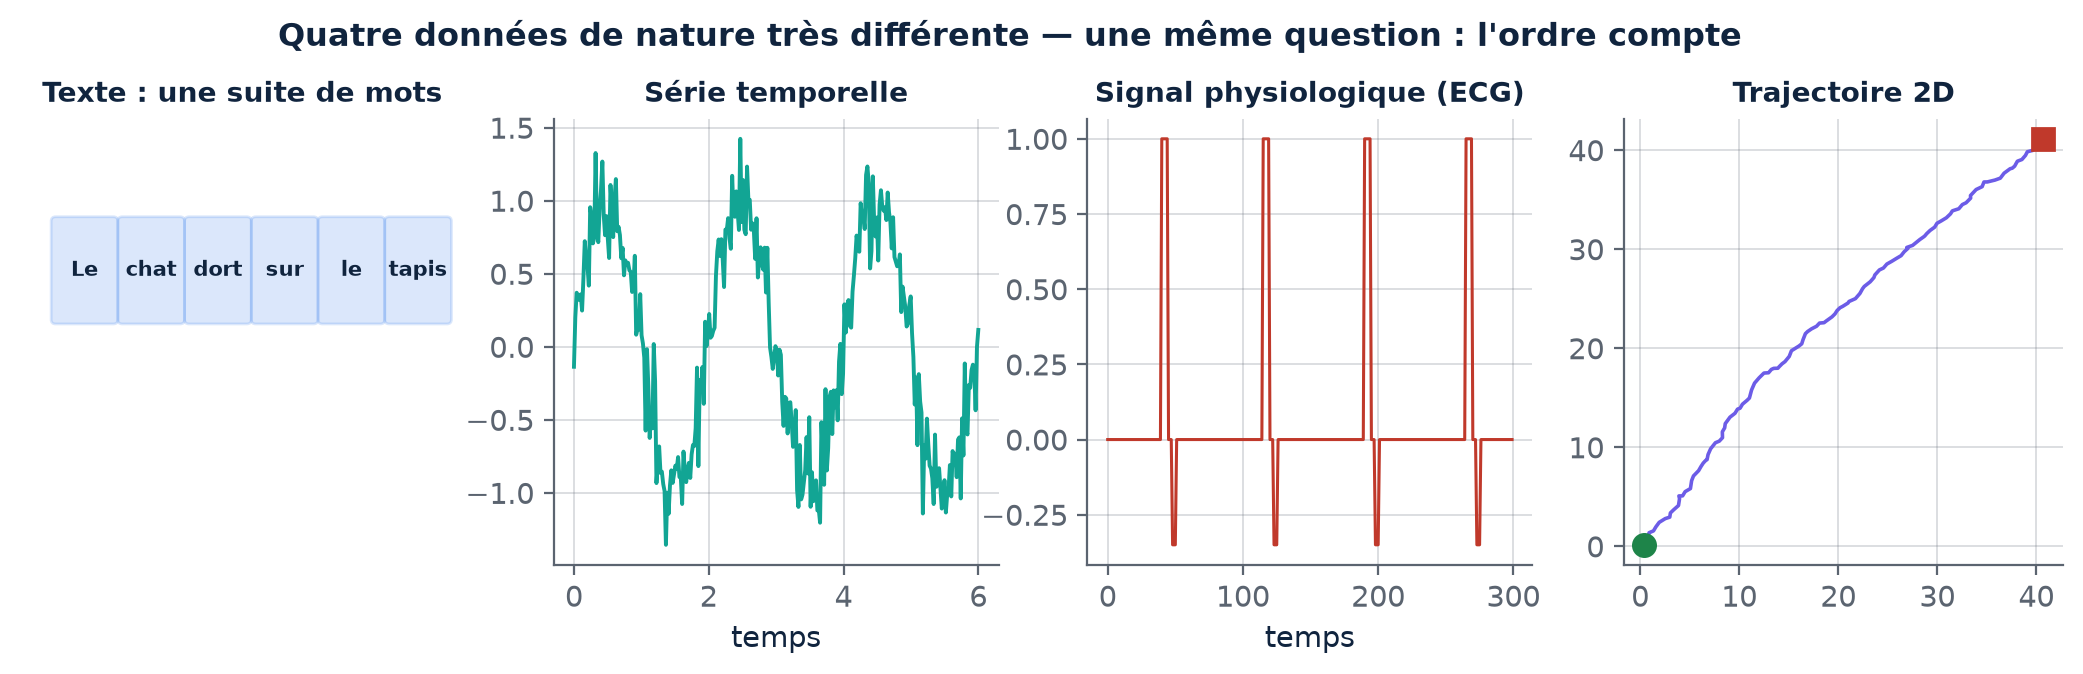
\includegraphics[width=\textwidth]{r01_types_sequences.png}
\end{column}
\begin{column}{0.42\textwidth}
\begin{itemize}
  \item Un texte : une suite de \textbf{mots}.
  \item Une série temporelle : des \textbf{mesures} datées.
  \item Un signal physiologique : un ECG, un capteur.
  \item Une trajectoire : des positions successives.
\end{itemize}
\begin{kbox}[Le dénominateur commun]
Une liste \textbf{ordonnée} d'éléments dont la longueur n'est pas fixée
d'avance.
\end{kbox}
\end{column}
\end{columns}
\end{frame}

\begin{frame}{Même ordre, autre monde}
\begin{columns}[t]
\begin{column}{0.48\textwidth}
\begin{wbox}[Ce que l'on savait faire]
Le CNN prend une image de \textbf{taille fixe} ($28 \times 28$, $32 \times 32$)
et en tire une décision. Les pixels se comptent, la structure est une grille.
\end{wbox}
\begin{wbox}[Ce qui change ici]
\begin{itemize}
  \item La longueur \textbf{varie} d'un exemple à l'autre.
  \item L'ordre porte l'information.
  \item Un mot du début peut gouverner la fin.
\end{itemize}
\end{wbox}
\end{column}
\begin{column}{0.48\textwidth}
\begin{ebox}[Question directe]
Peut-on aplatir une phrase comme on aplatissait une image, et nourrir un MLP ?

\medskip
Non : il faudrait fixer une longueur maximale, et le réseau chercherait des
corrélations entre des positions arbitraires.
\end{ebox}
\end{column}
\end{columns}
\end{frame}

\begin{frame}{Le fil rouge : une trajectoire à prédire}
\begin{columns}[t]
\begin{column}{0.48\textwidth}
\centering
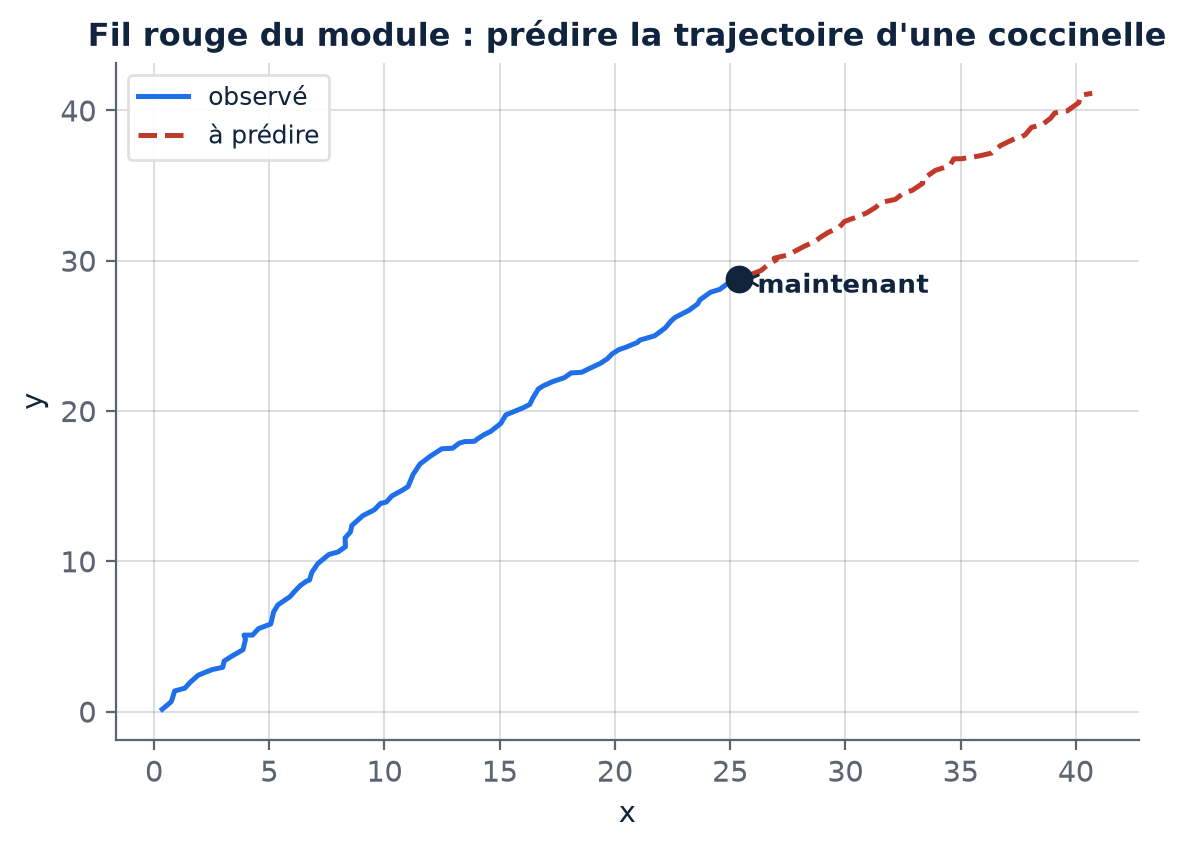
\includegraphics[width=0.46\textwidth]{r08_coccinelle.png}
\end{column}
\begin{column}{0.48\textwidth}
\begin{itemize}
  \item On observe 80 positions de la coccinelle.
  \item On veut prédire les 40 suivantes.
  \item Rien ne fixe la longueur d'avance : la séquence est \textbf{vivante}.
\end{itemize}
\begin{kbox}[Ce qui est demandé]
Utiliser le passé \textbf{comme un tout} --- pas comme une collection de points
indépendants.
\end{kbox}
\end{column}
\end{columns}
\end{frame}

\begin{frame}{Du texte aux nombres : le pipeline}
\begin{center}
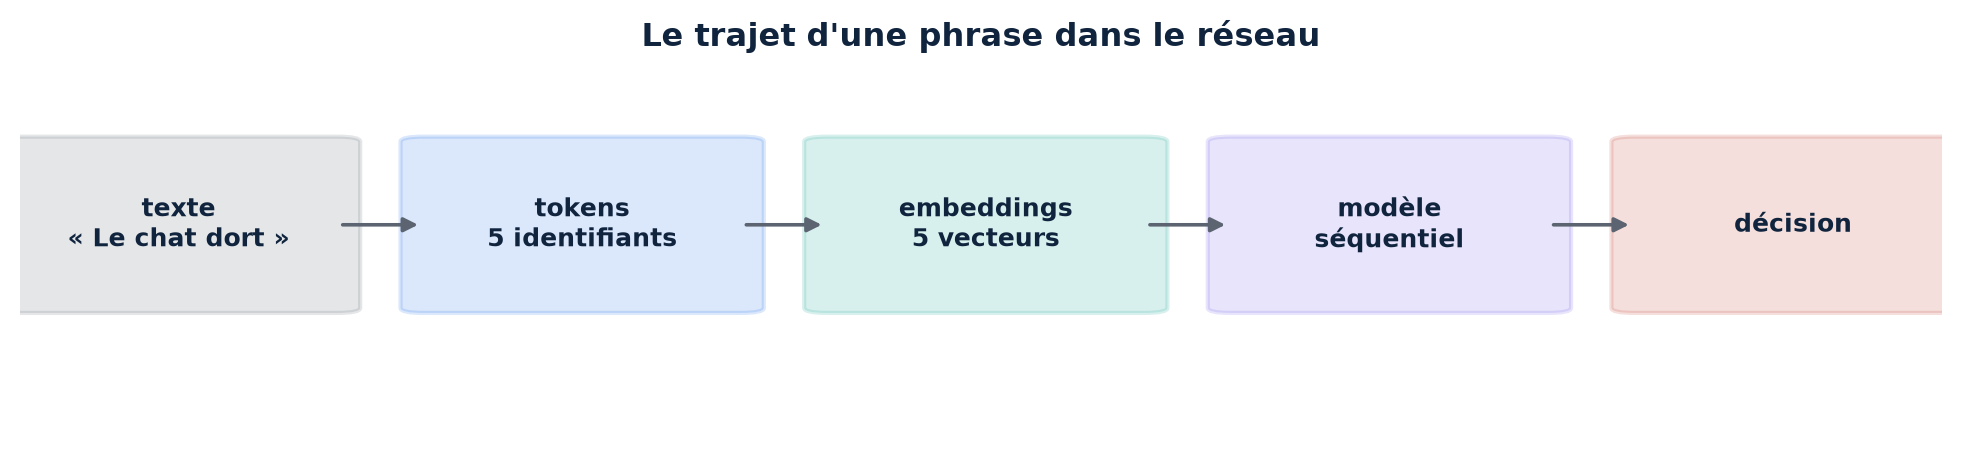
\includegraphics[width=0.94\textwidth]{r07_pipeline_sequence.png}
\end{center}
\vspace{1mm}
\begin{kbox}[Trois étapes obligatoires]
\begin{enumerate}
  \item \textbf{Tokeniser} : découper en unités (mots, sous-mots).
  \item \textbf{Indexer} : chaque unité devient un identifiant entier.
  \item \textbf{Plonger} : chaque identifiant devient un vecteur dense.
\end{enumerate}
\end{kbox}
\end{frame}

\begin{frame}{Quiz d'entrée}
\begin{qbox}[Question 1]
Laquelle de ces données n'est PAS séquentielle au sens de ce module ?
\begin{itemize}
  \item[(a)] une phrase \quad (b) un ECG \quad (c) une photo de chat
\end{itemize}
\end{qbox}
\begin{qbox}[Question 2]
« La souris mange le chat » et « Le chat mange la souris » contiennent les
mêmes mots. Un sac de mots les distingue-t-il ?
\begin{itemize}
  \item[(a)] oui, parfaitement \quad (b) non : l'ordre manque
\end{itemize}
\end{qbox}
\begin{qbox}[Question 3]
Pourquoi le padding est-il nécessaire dans un lot (batch) de séquences ?
\begin{itemize}
  \item[(a)] Pour accélérer \quad (b) Pour donner aux tenseurs une longueur commune
  \quad (c) Pour normaliser
\end{itemize}
\end{qbox}

% [fix] bloc deplace
\end{frame}
\begin{frame}{Quiz d'entrée (suite)}
\begin{solbox}[Réponses]
\textbf{1.} (c) : une image a une taille fixe, pas une suite ordonnée de longueur libre. \quad
\textbf{2.} (b) : le sac de mots détruit l'ordre, donc le sens. \quad
\textbf{3.} (b) : un tenseur doit être rectangulaire ; le masque neutralise le remplissage.
\end{solbox}
\end{frame}
